\documentclass[handout]{beamer}
\usepackage{amsmath,amssymb,amsthm,array}
\usepackage{bm}
\usepackage{multirow}
\usepackage{multicol}
\usepackage{algorithm}
\usepackage{algorithm2e}
\usepackage{hyperref}
\usepackage{algorithmic}
\usepackage[normalem]{ulem}
\usepackage{fontspec}
\usepackage{numprint}
\usepackage{mathtools}
\DeclarePairedDelimiter{\ceil}{\lceil}{\rceil}
\DeclarePairedDelimiter\floor{\lfloor}{\rfloor}

\setmainfont{CMU Serif}
\setsansfont{CMU Sans Serif}
\newfontfamily{\greekfont}{CMU Serif}
\newfontfamily{\greekfontsf}{CMU Sans Serif}

\usetheme{metropolis}

\setbeamertemplate{navigation symbols}{}

\title{Κρυπτοσυστήματα Διακριτού Λογαρίθμου}
\author{Παναγιώτης Γροντάς - Άρης Παγουρτζής}
\date{27/11/2018}
\defbeamertemplate*{footline}{shadow theme}
{%
  \leavevmode%
  \hbox{
		\begin{beamercolorbox}[wd=.4\paperwidth,ht=2.5ex,dp=1.125ex,leftskip=.3cm,rightskip=.3cm plus1fil]{title in head/foot}%
			\usebeamerfont{title in head/foot} Κρυπτοσυστήματα Διακριτού Λογαρίθμου  %
		\end{beamercolorbox}
		\begin{beamercolorbox}[wd=.5\paperwidth,ht=2.5ex,dp=1.125ex,leftskip=.3cm,rightskip=.3cm plus1fil]{title in head/foot}%
			\usebeamerfont{title in head/foot} \hfill \insertsection  %
		\end{beamercolorbox}
		\begin{beamercolorbox}[wd=.1\paperwidth,ht=2.5ex,dp=1.125ex,leftskip=.3cm plus1fil,rightskip=.3cm]{author in head/foot}%
			\usebeamerfont{author in head/foot}\insertframenumber\,/\,\inserttotalframenumber
		\end{beamercolorbox}%
  }%
  \vskip0pt%
}
\institute{ΕΜΠ - Κρυπτογραφία (2018-2019)}

 \hypersetup{
  pdfauthor={Panagiotis Grontas},
  pdftitle={EG},
  colorlinks=true,
  urlcolor=blue,
  pdfborderstyle={/S/U/W 1}	% border style will be underline of width 1pt
}



\begin{document}

\setlength{\columnseprule}{0.4pt}

\newcommand{\xor}{ \oplus }
\newcommand{\MSG}{ \mathtt{M} }
\newcommand{\KEY}{ \mathtt{K} }
\newcommand{\CPH}{ \mathtt{C} }
\newcommand{\keygen}{\mathtt{KeyGen}}
\newcommand{\enc}{\mathtt{Encrypt}}
\newcommand{\dec}{\mathtt{Decrypt}}
\newcommand{\adv}{$\mathcal{A}$ }
\newcommand{\advb}{$\mathcal{B} \,$ }
\newcommand{\chal}{$\mathcal{C} \,$ }
\newcommand{\hash}{$\mathcal{H} \,$ }
\newcommand{\cs}{$\mathcal{CS} \,$ }
\newcommand{\zns}{  \mathbb{Z}^*_n }
\newcommand{\zn}[1]{  \mathbb{Z}^*_#1 }

\newcommand{\green}[1]{\textcolor{teal}{#1}}
\newcommand{\Green}[1]{\textcolor{Teal}{#1}}
\newcommand{\ForestGreen}[1]{\textcolor{ForestGreen}{#1}}
\newcommand{\blue}[1]{\textcolor{blue}{#1}}
\newcommand{\magenta}[1]{\textcolor{magenta}{#1}}
\newcommand{\cyan}[1]{\textcolor{cyan}{#1}}

\newcommand{\twopartdef}[4]
{ 
		\begin{cases}
			#1 , #2 \\
			#3 , #4
		\end{cases} 
}

\npthousandsep{ }
\begin{frame}
\titlepage
\end{frame}



\begin{frame}{Περιεχόμενα}
\begin{itemize}
\item Διακριτός Λογάριθμος: Προβλήματα και Αλγόριθμοι
\item Το κρυπτοσύστημα ElGamal (Ορισμός, Ασφάλεια, Παραλλαγές)
\item Σχήματα Δέσμευσης με βάση το DLP
\item Διαμοιρασμός απορρήτων - Shamir Secret Sharing - Threshold ElGamal
\end{itemize}
\end{frame}


\section{DLP}
\begin{frame}{Προβλήματα Διακριτού Λογαρίθμου - (Υπενθύμιση)}

\begin{block}{DLP - Το πρόβλημα του Διακριτού Λογαρίθμου}
Δίνεται μια κυκλική ομάδα $\mathbb{G}=\langle g \rangle$ τάξης $q$ και ένα τυχαίο στοιχείο $y \in \mathbb{G}$

Να υπολογιστεί $x \in \mathbb{Z}_q$ ώστε $g^x = y$ δηλ. το $log_g y \in \mathbb{Z}_q$
\end{block}

\pause
\begin{block}{CDHP - Το υπολογιστικό πρόβλημα Diffie Hellman}
Δίνεται μια κυκλική ομάδα $\mathbb{G}=\langle g \rangle$, δύο στοιχεία $y_1=g^{x_1}, y_2 = g^{x_2}$

Να υπολογιστεί το $g^{x_1 \cdot x_2}$ 
\end{block}

\pause
\begin{block}{DDHP - Το πρόβλημα απόφασης Diffie Hellman}
	Δίνεται μια κυκλική  ομάδα $\mathbb{G}=\langle g \rangle$, δύο στοιχεία $y_1=g^{x_1}, y_2 = g^{x_2}$ και κάποιο  $y \in \mathbb{G}$ 
	
	Να εξεταστεί αν  $y = g^{x_1 \cdot x_2}$  ή ισοδύναμα \\
	
	μπορούμε να ξεχωρίσουμε τις τριάδες ($g^{x_1}, g^{x_2}, g^{x_1x_2}$) και  ($g^{x_1}, g^{x_2}, y$);
\end{block}

\end{frame}
 

\begin{frame}{Σχέσεις Προβλημάτων - (Υπενθύμιση)}
\begin{block}{$CDHP \leq DLP$}
Αν μπορούμε να λύσουμε το $DLP$, τότε μπορούμε να υπολογίζουμε τα $x_1, x_2$ από τα $y_1, y_2$ και στην συνέχεια το $g^{x_1 \cdot x_2}$
\end{block}

\pause
 
\begin{block}{$DDHP \leq CDHP$}
Αν μπορούμε να λύσουμε το $CDHP$, υπολογίζουμε το $g^{x_1 \cdot x_2}$ και ελέγχουμε ισότητα με το $y$
\end{block}
 
\pause 
Δηλαδή: $DDHP \leq CDHP \leq DLP$
\end{frame}
 
 

\begin{frame}{Random Self - Reducibility}
	\begin{block}{Θεώρημα}
		'Εστω ομάδα $\mathbb{G}$ τάξης $q$ και $g \in G$. Έστω $A$ PPT αλγόριθμος με την εξής ιδιότητα:
		$$u \in_R \mathbb{G} : Pr[A(u)=DL(u)] = \epsilon$$
		Υπάρχει PPT αλγόριθμος $B$ με την ιδιότητα:
		$$\forall u \in \mathbb{G}, B(u) \in \{fail,x\} \land Pr[x=DL(u)] = \epsilon$$
	\end{block}
\end{frame}

\begin{frame}{Random Self - Reducibility}
	\begin{block}{Απόδειξη}
		Ο αλγόριθμος $B$ είναι ο εξής:
		\begin{algorithm}[H]
		{Είσοδος $u \in \mathbb{G}$} \; 

		{$\sigma \leftarrow_R \mathbb{Z}_q$} \; 

		{$u_1 \leftarrow u \cdot g^\sigma$} \; 

		{$a_1 \leftarrow  A(u_1)$}\; 

		\eIf{$g^{a_1} \neq u_1$}{return fail}{return {$a_1 - \sigma$}} \;
		\end{algorithm}
	\end{block}
\end{frame}

\begin{frame}{Random Self - Reducibility (Παρατηρήσεις)}
	Με $n \cdot \ceil{\frac{1}{\epsilon}}$ επαναλήψεις η πιθανότητα επιτυχίας είναι:
	$$Pr[B(u)=DL(u)] = 1 - (1-\epsilon)^{n \cdot \ceil{\frac{1}{\epsilon}}} \geq  1-e^{-n}$$

	\emph{Συμπέρασμα}: Εύκολο DLP για μη αμελητέο ποσοστό τυχαίων στοιχείων, εύκολο για όλα τα στοιχεία της ομάδας

	\emph{Συνέπεια}: Κατάλληλα 'Δύσκολα΄' προβλήματα για κρυπτογραφία: Δύσκολα στη χειρότερη περίπτωση και Random Self - Reducible (δύσκολα στη μέση περίπτωση) 
	
	\alert{Δεν ισχύει για όλα τα NP-hard προβλήματα} 

\end{frame}

\begin{frame}{Επιλογή Ομάδας}
	\begin{itemize}
		\item Καθορίζει τη δυσκολία του προβλήματος 
		\item Δύο επιλογές:
		\begin{itemize}
			\item $(\mathbb{Z}_p^*, \cdot)$ με $p$ πρώτο (σε υποομάδα)
			\item Λόγοι:
			\begin{itemize}
				\item Δυσκολότερο το DLP
				\item Τετριμμένη εύρεση γεννήτορα (όλα τα στοιχεία εκτός από το 1)
				\item Εύκολη εύρεση αντίστροφου
			\end{itemize}
			\item $(\mathcal{E}(\mathbb{F}_p),+)$ (Ελλειπτικές καμπύλες: 'Λογάριθμος' αφορά πρόσθεση)
			\begin{itemize}
				\item ίδια επίπεδα ασφάλειας με μικρότερη τιμή παραμέτρου ασφάλειας
			\end{itemize}
		\end{itemize}  
	\end{itemize}
	\end{frame}

\begin{frame}{Αλγόριθμοι DL}
\begin{block}{Brute Force}
Για ομάδα $\mathbb{G}=\langle g \rangle$ τάξης $q$ $\lambda$ bits
\medskip

Δοκιμή όλων των $x \in \mathbb{Z}_q$ μέχρι να βρεθεί τέτοιο ώστε $g^x = y$
\medskip

Πολυπλοκότητα $O(2^\lambda)$

Γενικευμένη μέθοδος - δεν εξαρτάται απο χαρακτηριστικά ομάδας
\end{block}
\end{frame}

%\begin{frame}{Σχέση με γεννήτορα}
%\begin{block}{Η δυσκολία του DLP είναι ανεξάρτητη από την επιλογή του γεννήτορα}
%Έστω $g_1, g_2$ γεννήτορες του $\mathbb{Z}_p^*$
%
%Για κάποιο $y \in \mathbb{Z}_p^*$: $y = g_1^x$ και $y=g_2^z$
%
%Δηλαδή: $g_1^x = g_2^z=(g_1^w)^z$
%
%Άρα: $x = wz \pmod{p-1} \Rightarrow z = xw^{-1} \pmod{p-1}$
%
%\end{block}
%Αν το DLP,μπορεί να επιλυθεί σε μία βάση - γεννήτορα, τότε μπορεί να υπολογιστεί σε οποιαδήποτε.
%\end{frame}

\begin{frame}{Αλγόριθμος Baby step - Giant Step (Shanks)}
Αλγόριθμος \green{Meet-In-The Middle}
\begin{itemize}
\item Στόχος: εύρεση $x:$ $y=g^x$
\item Βασική ιδέα:  $\forall x \in \mathbb{Z}, \exists k,a,b \in \mathbb{Z} :  \, \,  x = ak+b,  $ 
\pause
\item $y = g^x \Rightarrow y=g^{ak} \cdot g^{b} \Rightarrow \green{{y}{g^{-ak}}=g^{b}}$
\pause
\item Θα υπολογίζουμε $g^b$ και $yg^{-ak}$ μέχρι να συναντηθούν
\pause
\begin{enumerate}
\item Ξεκινάμε στη `μέση': $k = \ceil{\sqrt{q}}$\pause
\item \textbf{Baby steps - μέγεθος $1$}: \\Υπολογίζουμε $g^b, b \in \{0, 1, \cdots, k-1 \}$ και αποθηκεύουμε \pause
\item \textbf{Giant steps - μέγεθος $k$}:\\ Υπολογίζουμε ${yg^{-ak}}, a \in \{0, 1, \cdots, k-1 \}$ και το αναζητούμε στα αποτελέσματα του Βημ. 2 \pause
\item Όταν βρεθεί υπολογίζουμε: $x = ak+b$
\end{enumerate}
\end{itemize}
\begin{small}
Πολυπλοκότητα Χρόνου: $O(2^\frac{\lambda}{2})$ - \alert{Βέλτιστη} για γενικευμένο \\
Πολυπλοκότητα Χώρου: $O(2^\frac{\lambda}{2})$ -  Βέλτιστη αυτή του \alert{Pollard rho} σταθερή
\end{small}
\end{frame}

\begin{frame}{Παράδειγμα Baby step - Giant Step}
\begin{block}{Θέλουμε το $2^x = 17 \pmod{29}$ στο $\mathbb{Z}_{29}^*=\langle 2 \rangle$, $\ceil{\sqrt{29}} = 6$}
\begin{columns}
\column{0.5\textwidth}
\begin{itemize}
\item $b \in \{0 \cdots 5\}$
\item $2^{0} = 1  \pmod{29}$
\pause
\item $2^{1} = 2  \pmod{29}$
\pause
\item $2^{2} = 4 \pmod{29}$
\pause
\item $2^{3} = 8  \pmod{29}$
\pause
\item $2^{4} = 16  \pmod{29}$
\pause
\item $2^{5} = 3  \pmod{29}$
\end{itemize}
\pause
\column{0.5\textwidth}

\begin{itemize}
\item $a \in \{0 \cdots 5\}$
\item $17 \cdot 2^{-0 \cdot 6} = 17  \pmod{29}$
\pause
\item $17 \cdot 2^{-1 \cdot 6} = 37  \pmod{29}$
\pause
\item $17 \cdot 2^{-2 \cdot 6} = 19  \pmod{29}$
\pause
\item $17 \cdot 2^{-3 \cdot 6} = \green{8}  \pmod{29}$
\item Βρέθηκε
\end{itemize}
\end{columns}
\pause
\begin{center}
Άρα $x = 18+3 = 21$\\
Πράγματι: \green{$2^{21} = 17 \pmod{29}$}
\end{center}
\end{block}

\end{frame}

\begin{frame}{Αλγόριθμος Pohlig-Hellman - Ιδέα}

\begin{block}{Παρατήρηση}
Η δυσκολία του DLP σε μια ομάδα $\mathbb{G}$ εξαρτάται από τη δυσκολία του στις διάφορες υποομάδες της.
\end{block}
\pause
\begin{block}{Συγκεκριμένα}
Παραγοντοποίηση της τάξης 

(πχ. στο $\mathbb{Z}_p^*$: $p-1 = \prod_{i=1}^m p_i^{e_i}$ με $p_i$ πρώτο)

Επίλυση DLP σε κάθε υποομάδα και συνδυασμός με CRT 
\end{block}
\pause
\begin{block}{Smooth Number}
Μπορεί να παραγοντοποιηθεί σε μικρούς πρώτους - Αν ισχύει για την τάξη επιταχύνει σημαντικά τον αλγόριθμο
\end{block}
\end{frame}

\begin{frame}{Αλγόριθμος Pohlig-Hellman} 
\begin{small}
\begin{itemize}
\item Παραγοντοποιούμε την τάξη: $p-1 = \prod_{i=1}^m p_i^{e_i}$ \pause
\item Για κάθε $p_i$ γράφουμε  $x = a_0+a_1 p_i+\cdots+a_{e_i-1}p_i^{e_i-1} \pmod{p_i^{e_i}}$ με $a_j \in \{0,\cdots,p_{i}-1\}$
\item Θα υπολογίσουμε τους συντελεστές ως εξής: 
\item Για το $a_0$ ισχύει: $y^\frac{p-1}{p_i} = g^{a_0\frac{p-1}{p_i}} \pmod{p}$ (1) επειδή:
 \begin{align*} y^\frac{p-1}{p_i} = (g^{x})^{\frac{p-1}{p_i}} = g^{ (a_0+a_1 p_i+\cdots+a_{e_i-1}p_i^{e_i-1}) \frac{p-1}{p_i}}  =\\  
	 g^{ (a_0+Kp_i) \frac{p-1}{p_i}} = g^{ a_0 \frac{p-1}{p_i}} g^{ Kp_i \frac{p-1}{p_i}}  = \\
	 g^{a_0\frac{p-1}{p_i}} \pmod{p} \end{align*} \pause
\item Υπολογισμός $a_0$ (πχ. με αλγόριθμο Shanks) 
\end{itemize}
\end{small}
\end{frame}

\begin{frame}{Αλγόριθμος Pohlig-Hellman} 
\begin{small}
\begin{itemize}
\item Για τον υπολογισμό των υπόλοιπων συντελεστών:
\begin{itemize}
	\item Δημιουργούμε ακολουθία $\{ y_j \}$ με $y_0=y$ και
	\item $y_{j} = y_{j-1} \cdot g^{-(a_0+a_1p_i+\cdot+a_{j-1}{p_i}^{j-1})} \pmod{p}$
	\item Γενικεύοντας την (1) έχουμε: $y_{j}^\frac{p-1}{p_i^{j+1}} = g^{a_j \frac{p-1}{p_i}}$ 
	\item Yπολογίζουμε το $a_j$
\end{itemize}  
\item Συνδυασμός λύσεων με CRT  
\end{itemize}
\end{small}
\end{frame}

\begin{frame}{Pohlig-Hellman - παράδειγμα}
\begin{block}{Θέλουμε το $2^x = 17 \pmod{29}$ στο $\mathbb{Z}_{29}^*=\langle 2 \rangle$}
Παραγοντοποιούμε την τάξη: $28=2^2 7$ \\
$x_2 = a_0 + 2a_1 \pmod{4}$ και \\ 
$x_7 = a_0 \pmod{7}$ \\
\end{block}

\pause
\begin{block}{Υπολογισμός $a_0$ για το $x_2$}
$y^\frac{p-1}{2} = g^{a_0 \frac{p-1}{2}} \Rightarrow 17^{14} = 2^{14 a_0} \Rightarrow  2^{14 a_0} = 28 = -1 \pmod{29}$ \\
Άρα $a_0=1$
\end{block}

\pause
\begin{block}{Υπολογισμός $y_1$ για το $x_2$}
$y_1 = y g^{-a_0} = 17 \cdot 2^{-1} = 17 \cdot 15 = 23 \pmod{29} $
\end{block}
\end{frame}

\begin{frame}{Pohlig-Hellman - παράδειγμα}
\begin{block}{Υπολογισμός $a_1$ για το $x_2$}
$y_1^\frac{p-1}{4} = g^{a_1 \frac{p-1}{2}} \Rightarrow 23^7  = 2^{14 a_1} \Rightarrow 2^{14 a_1} = 1 \pmod{29}$\\
Άρα $a_1=0$ \\
\end{block}
Άρα \green{$x_2 = 1 + 0 = 1\pmod{4}$}
\pause
\begin{block}{Υπολογισμός $a_0$ για το $x_7$}
$y^\frac{p-1}{7} = g^{a_0 \frac{p-1}{7}} \Rightarrow 17^4 = 2^{4 a_0} \Rightarrow  2^{4 a_0} = 1 \pmod{29}$ \\
Άρα $a_0=0$
\end{block}
Άρα \green{$x_7 = 0 \pmod{7}$}

\pause
Από $x_2 = 1 + 0 = 1\pmod{4}$ και $x_7 = 0 \pmod{7}$ με CRT προκύπτει $x = 21$
 
\end{frame}

\begin{frame}{Δυσκολία DDHP}

\begin{block}{Θεώρημα}
To DDHP δεν είναι δύσκολο στην $\mathbb{Z}_p^*$
\end{block}
 
Μπορεί να κατασκευαστεί αποδοτικός αλγόριθμος διαχωρισμού τριάδας DH $g^a,g^b,g^{ab}$ από μια τυχαία τριάδα $g^a,g^b,g^c$.\\
\pause
\magenta{Πώς:} Χρησιμοποιώντας το \green{σύμβολο Legendre.}
 
\begin{block}{To σύμβολο Legendre διαρρέει το DLP parity}
Από τον ορισμό: 
$(\frac{g^{x}}{p}) = (g^{x})^{\frac{p-1}{2}}$ \\ \pause
Όμως: $g^{p-1} = 1 \pmod{p}$  \pause \\ 
Άρα: 
$g^\frac{p-1}{2} = -1 \pmod{p}$ \pause\\
Δηλαδή:
$(\frac{g^{x}}{p}) = (-1)^x$ \pause\\
Αν $x$ μονός  τότε $(\frac{g^{x}}{p}) = -1$  \\ \pause
Αν $x$ ζυγός  τότε $(\frac{g^{x}}{p}) = 1$   
\end{block}
\end{frame}

\begin{frame}{Δυσκολία DDHP}
\begin{small}
Για τυχαία τριάδα: $Prob[(\frac{g^{c}}{p}) = 1] = \frac{1}{2}$ \\
\pause
Για τριάδα DH: $Prob[(\frac{g^{ab}}{p}) = 1] = \frac{3}{4}$
\pause 

	\begin{algorithm}[H]
	Υπολόγισε $(\frac{g^{a}}{p}),(\frac{g^{b}}{p}),(\frac{g^{c}}{p})$\;

	\eIf{$(\frac{g^{c}}{p}) = 1 \land ((\frac{g^{a}}{p}) =1 \lor (\frac{g^{b}}{p}) = 1))$}{Επιστροφή "Τριάδα Diffie Hellman"}{Επιστροφή "Τυχαία Τριάδα"}
	\caption{Ο αλγόριθμος διαχωρισμού}
  \end{algorithm}

\pause
Πλεονέκτημα: $\frac{3}{8}$ (γιατί;) \\

\alert{ΜΗ ΑΜΕΛΗΤΕΟ}\\
\end{small}
\end{frame}

\begin{frame}{Επιλογή του $\mathbb{G}$}
\begin{small}
\begin{block}{Συνέπειες}
Δουλεύουμε σε μεγάλη υποομάδα του $\mathbb{Z}_p^*$ με τάξη πρώτο $q$
\end{block}
\pause
\begin{block}{Για παράδειγμα:}
Επιλογή safe prime: $p = 2q+1$ με $q$ πρώτο 

Δουλεύουμε στην υποομάδα τετραγωνικών υπολοίπων τάξης $q$

Επιλογή schnorr primes $p = k \cdot q+1$ με $q$ πρώτο

\alert{Παρ' όλα αυτά}: Yποεκθετικοί αλγόριθμοι (index calculus)
\end{block}
\pause
\begin{block}{Μεγέθη}
\begin{tabular}{ccc}
Symmetric Security & $|p|$ & $|q|$ \\
80 bits &  1024 & 160 \\
112 bits & 2048 & 224 \\
128 bits &  3072 & 256 \\
192 bits &  7680 & 384 \\
256 bits &  15360 & 512 \\
\end{tabular}
\end{block}
\end{small}
\end{frame} 

\section{Το κρυπτοσύστημα ElGamal}
\begin{frame}{Ορισμός ElGamal}
 
\textbf{Δημιουργία Κλειδιών:}
$KeyGen(1^{\lambda}) = (y=g^x,x)$
\begin{itemize}
\item Επιλογή δύο μεγάλων πρώτων $p,q$ ώστε $q \mid (p-1)$  
\item $\mathbb{G}$: υποομάδα τάξης q του $\mathbb{Z}_p^*$ - $g$ γεννήτορας 
\item Ιδιωτικό κλειδί: τυχαίο $x \in \mathbb{Z}_q$
\item Δημόσιο κλειδί: $y = g^x \bmod{p}$
\item Επιστροφή $(y,x)$
\end{itemize}
\pause
 
\textbf{Κρυπτογράφηση} 
\begin{itemize}
\item Επιλογή τυχαίου $r \in \mathbb{Z}_q$
\item $\enc_y(r,m) = (g^r \bmod p, m \cdot y^r \bmod p)$
\end{itemize}
\pause

\textbf{Αποκρυπτογράφηση}
\begin{itemize}
\item $\dec_x(a,b) = \frac{b}{a^x}$
\end{itemize} 
\pause
 
\magenta{Ορθότητα} $\dec_x(\enc_y(r,m))= \frac{m y^r}{(g^r)^x} = m$
 
\end{frame}

\begin{frame}{Πρακτικά Θέματα}

\green{Πιθανοτική Κρυπτογράφηση:} Ένα μήνυμα έχει πολλά πιθανά κρυπτοκείμενα \\
\pause
\alert{Message expansion} Κρυπτοκείμενο διπλάσιο του μηνύματος \\
\pause
\begin{block}{Επιτάχυνση Κρυπτογράφησης}
Κόστος: 2 υψώσεις σε δύναμη - 1 πολλαπλασιασμός\\
Ύψωση σε δύναμη:Δεν εξαρτάται από το μήνυμα (precomputation)
\end{block}

\end{frame}

\begin{frame}{Ασφάλεια Κρυπτογράφησης}
\begin{block}{\textbf{Μυστικότητα} ElGamal \equiv Ασφάλεια CDHP}
Αντιστοιχία δημοσίων στοιχείων
\begin{align*}
g^{x_1} \equiv g^r  \\
g^{x_2} \equiv y=g^x \\
g^{x_1x_2} \equiv y^r
\end{align*}
\pause
$EG \leq CDHP$: $CDHP \Rightarrow$ \pause Υπολογισμός $g^{x_1x_2} = y^r$ \pause $\Rightarrow$ αποκρυπτογράφηση (με εύρεση αντιστρόφου του $y^r$)\\
\pause
$CDHP \leq EG$: $EG \Rightarrow$ \pause\\
 Για οποιοδήποτε $c \in \mathbb{G}$: \\ \pause 
 εύρεση $m$ που αντιστοιχεί στο $g^{x_2},(g^{x_1},c)$ (χρήση EG ως oracle αποκρυπτογράφησης με δημόσιο κλειδί $g^{x_2}$) \\ \pause 
 Yπολογισμός $g^{x_1x_2} = \frac{c}{m}$ 
\end{block}

\end{frame}

\begin{frame}{Επανάληψη τυχαιότητας $\rightarrow$ Επίθεση KPA}
KPA: Γνωρίζουμε  ζεύγη μηνυμάτων - κρυπτοκειμένου για τα οποία έχει χρησιμοποιηθεί η ίδια τυχαιότητα
\pause
\begin{block}{Επίθεση}
$(c_r,c_1) = \enc_y(r,m_1) = (g^r \bmod p, m_1 \cdot y^r \bmod p)$
$(c_r,c_2) = \enc_y(r,m_2) = (g^r \bmod p, m_2 \cdot y^r \bmod p)$
\end{block}
\pause
Αν γνωρίζω το $(m_1,c_1)$:
$c_1 = m_1 \cdot y^r \bmod p \Rightarrow y^r = c_1 \cdot m_1^{-1}$\\
\medskip
\pause
Μπορώ να υπολογίσω το $m_2$ ως:
$m_2 = \frac{c_2}{y^r} = \frac{c_2}{c_1 \cdot m_1^{-1}}$
\end{frame}

\begin{frame}{Ασφάλεια σε επιθέσεις CPA}
\begin{block}{Θεώρημα}
Αν το DDHP είναι δύσκολο, τότε το κρυπτοσύστημα El Gamal διαθέτει ασφάλεια IND-CPA.
\end{block}

Απόδειξη:

Έστω ότι το ElGamal δεν διαθέτει ασφάλεια IND-CPA. 

Άρα $\exists$ \adv, ο οποίος μπορεί να νικήσει στο παιχνίδι CPA με μη αμελητέα πιθανότητα. 

Κατασκευή \advb:
\begin{itemize}
\item Είσοδος: τριάδα στοιχείων
\item Εσωτερικά: Προσομοίωση του \chal στο παιχνίδι CPA και χρήση \adv 
\item Αποτέλεσμα: Ξεχωρίζει DH τριάδα από τυχαία 
\end{itemize}
\end{frame}

\begin{frame}{Ασφάλεια σε επιθέσεις CPA}
	\begin{center}
	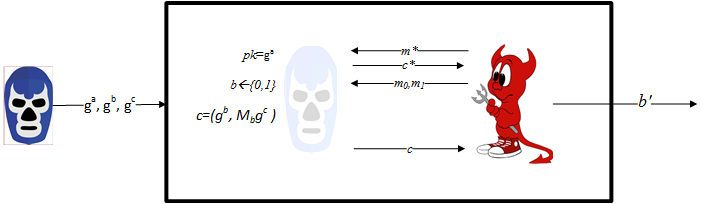
\includegraphics[scale=.6]{egcpa.png}
	\end{center}
	\end{frame}

\begin{frame}{Ασφάλεια σε επιθέσεις CPA}
\begin{itemize}
\item Είσοδος: $g^\alpha,g^\beta, g^c$
\item Στο CPA-GAME δημόσιο κλειδί $y =  g^\alpha$ 
\item Ο \advb απαντά στις κρυπτογραφήσεις του \adv
\item Όταν ο \adv προκαλέσει με δύο μηνύματα 
\begin{itemize}
\item o \chal διαλέγει τυχαίο $bit \in \{0, 1\}$,
\item κρυπτογραφεί το $M_b$ με τυχαιότητα το $g^\beta$ και πολλαπλασιάζει με $g^{c}$
\item Τελικά στέλνει το:  $( g^\beta  , M_b \cdot g^{c}  )$
\end{itemize}
\item O \adv επιστρέφει την τιμή του ${bit}^*$
\item Ο \advb εξάγει το ${bit}^*$
\end{itemize}


\end{frame}

\begin{frame}{Ασφάλεια σε επιθέσεις CPA}
\begin{block}{Ανάλυση}
\begin{itemize}

\item Για τριάδα DH: $g^c = (g^\alpha)^\beta = y^\beta $ 
\begin{itemize}
	\item ο \adv θα λάβει ένα έγκυρο κρυπτοκείμενο ElGamal.
	\item H πιθανότητα να μαντέψει σωστά είναι τουλάχιστον: ${1}/{2} + \text{non-negl}(\lambda)$. 
\end{itemize}


\item Για τυχαία τριάδα: ο \adv θα πρέπει να μαντέψει τυχαία
\item Πιθανότητα επιτυχίας: $\frac{1}{2}$.

\item Τελική πιθανότητα επιτυχίας για \advb τουλάχιστον $\text{non-negl}(\lambda)$
\item Μπορεί να ξεχωρίσει μία DH τριάδα από μία τυχαία με μη αμελητέα πιθανότητα.

\end{itemize}
\end{block}
\end{frame}

\begin{frame}{Ομομορφικές Ιδιότητες}

\begin{block}{Πολλαπλασιαστικός Ομομορφισμός}
\begin{align*}
\enc_y(r_1,m_1) \cdot \enc_y(r_2,m_2) = \\
(g^{r_1}, m_1 y^{r_1}) \cdot (g^{r_2}, m_2 y^{r_2}) =\\
(g^{r_1+r_2}, (m_1 \cdot m_2) \cdot y^{r_1+r_2}) = \\
\enc_y( r_1+r_2,m_1  m_2)
\end{align*}
\end{block}

\end{frame}

\begin{frame}{Ομομορφικές Ιδιότητες}

\begin{block}{Reencryption}
\begin{align*}
\enc_y(r_1,m) \cdot \enc_y(r_2,1) = \\
(g^{r_1}, my^{r_1}) \cdot (g^{r_2},  y^{r_1}) =\\
(g^{r_1+r_2}, my^{r_1+r_2}) =
\enc_y(r_1+r_2,m) 
\end{align*}
\end{block}
\green{Αλλαγή της τυχαιότητας - Αλλαγή της μορφής του μηνύματος} \\
\alert{...χωρίς γνώση του ιδιωτικού κλειδιού} \\
\alert{Malleability}

\end{frame}

\begin{frame}{Ομομορφικές Ιδιότητες}

\begin{block}{Προσθετικός Ομομορφισμός - Εκθετικό ElGamal}
Κρυπτογράφηση του $g^m$ αντί για $m$

$\enc_y(r,m) = (g^r, g^m y^r)$

\begin{align*}
  \enc_y(r_1,m_1) \cdot \enc_y(r_2,m_2) = \\
(g^{r_1}, g^{m_1} y^{r_1}) \cdot  (g^{r_2}, g^{m_2} y^{r_2}) =\\
(g^{r_1+r_2} , g^{m_1 + m_2} \cdot y^{r_1+r_2}) = \\
\enc_y(r_1+r_2,(m_1 + m_2))
\end{align*}

Αποκρυπτογράφηση: Λαμβάνουμε το $g^m$

\alert{Επίλυση διακριτού λογαρίθμου ('εύκολου')}.

\end{block}

\end{frame}

\begin{frame}{Ασφάλεια σε επιθέσεις CCA}
 
\begin{block}{To textbook ElGamal δεν διαθέτει CCA-security}
Έστω ότι ο \adv  μπορεί να αποκρυπτογραφήσει μηνύματα επιλογής του, εκτός του $c$.
\begin{itemize}
\item Στόχος: Αποκρυπτογράφηση του $c = (G,M) = (g^r, m_b y^r)$
\pause
\item Κατασκευή $c' = (G',M') = (G \cdot g^{r'}, M \cdot a y^{r'}) = (g^{r+r'}, a \cdot m_b \cdot y^{r+r'}) $, όπου $a$ επιλέγεται από τον  \adv 
\pause
\item H αποκρυπτογράφηση του $M'$ ($\frac{M'}{G'^x}$) δίνει το $am_b$ και κατά συνέπεια το $m_b$
\pause
\item Αν $m_b = m_0$ επιστρέφει $b^*=0$ αλλιώς επιστρέφει $b^*=1$
\end{itemize}
\end{block}
\end{frame}

\section{Cramer-Shoup cryptosystem}

\begin{frame}{ElGamal CCA2: Cramer-Shoup cryptosystem}
\begin{itemize}
\item Ronald Cramer, Victor Shoup, Crypto 1998 \pause
\item Επέκταση του ElGamal \pause
\item Χρήση συνάρτησης σύνοψης \hash (υπάρχουν εκδόσεις και χωρίς)
\item Αν ισχύει η υπόθεση DDH, τότε παρέχει IND-CCA2
\end{itemize}
\end{frame}

\begin{frame}{ElGamal CCA2: Cramer-Shoup cryptosystem}
\begin{block}{Δημιουργία Κλειδιών}
\begin{itemize}
\item Επιλογή πρώτων $p,q$ με $p=2q+1$ \pause
\item $\mathbb{G}$ ειναι η υποομάδα ταξης $q$ στο $\zn{p}$ \pause
\item Επιλογή random generators $g_1, g_2$ \pause

\item Επιλογή τυχαίων στοιχείων $x_1,x_2,y_1,y_2,z \in \mathbb{Z}_{q}$ \pause
\item Υπολογισμός
\begin{itemize} 
\item $c=g_1^{x_1}g_2^{x_2}$
\item $d=g_1^{y_1}g_2^{y_2}$
\item $h=g_1^{z}$
\end{itemize} \pause
\item Δημόσιο Κλειδί: $(c,d,h)$ \pause
\item Μυστικό Κλειδί: $(x_1,x_2,y_1,y_2,z)$ \pause
\end{itemize}
\end{block}

\end{frame}
\begin{frame}{ElGamal CCA2: Cramer-Shoup cryptosystem}

\begin{block}{Κρυπτογράφηση}
\begin{itemize}
\item Κωδικοποίηση μηνύματος $m$ στο $\mathbb{G}$ \pause
\item Επιλογή τυχαίου $r \in \mathbb{Z}_{q}$ \pause
\item Υπολογισμός
\begin{itemize} 
\item $u_1 = g_1^r,u_2 = g_2^r$ \pause
\item $e = m h^r$ \pause
\item $\alpha = $ \hash$(u_1||u_2||e)$ \pause
\item $v = c^r d^{r\alpha}$  \pause
\end{itemize}
\item Κρυπτογράφημα: $(u_1,u_2,e,v)$
\end{itemize}
\end{block}

\end{frame}
\begin{frame}{ElGamal CCA2: Cramer-Shoup cryptosystem} 
\begin{block}{Αποκρυπτογράφηση}
\begin{itemize}
\item Υπολογισμός $\alpha = $ \hash$(u_1||u_2||e)$ \pause
\item Έλεγχος αν $u_1^{x_1}u_2^{x_2}(u_1^{y_1}u_2^{y_2})^\alpha=v$. Σε περίπτωση αποτυχίας έξοδος χωρίς αποκρυπτογράφηση \pause
\item Σε περίπτωση επιτυχίας υπολογισμός $m = \frac{e}{u_1^z}$
\end{itemize}
\end{block}
\end{frame}

\begin{frame}{ElGamal CCA2: Cramer-Shoup cryptosystem}
\begin{block}{Ορθότητα}
$\frac{e}{u_1^z} = \frac{mh^r}{u_1^z} = m \cdot \frac{g_1^{zr}}{g_1^{rz}} = m$
\begin{itemize}
\item $h,z$ αντιστοιχούν σε δημόσιο - ιδιωτικό κλειδί  ElGamal \pause
\item $u_1, e$ αντιστοιχούν στο κρυπτογράφημα του ElGamal 
\end{itemize}
\end{block}
\pause
\begin{block}{Παρατηρήσεις}
\begin{itemize}
\item $u_2,v$ λειτουργούν ως έλεγχος ακεραιότητας, ώστε να  μπορεί να αποφευχθεί το malleability \pause
\item Διπλάσια πολυπλοκότητα από ElGamal τόσο σε μέγεθος κρυπτοκειμένου, όσο και σε υπολογιστικές απαιτήσεις
\end{itemize}
\end{block}
\end{frame}

\section{DLP-based Commitment Schemes}
\begin{frame}{DLP-based Commitment Schemes}
\begin{block}{Coin Flipping over the telephone}
\begin{itemize}
\item Η Alice και o Bob διαφωνούν (τηλεφωνικά) για το πού θα πάνε
\pause
\item Αποφασίζουν να ρίξουν δύο νομίσματα (απομακρυσμένα)
\pause
\item Ίδιο αποτέλεσμα: διαλέγει η Alice
\pause
\item Διαφορετικό Αποτέλεσμα: διαλέγει ο Bob
\pause
\item Προβλήματα;
\end{itemize}
\end{block}
\end{frame}

\begin{frame}{DLP-based Commitment Schemes}
\begin{block}{Λύση:  Commitment Schemes}
\begin{itemize}
\item Ιδιότητες
\pause
\begin{itemize}
\item \textbf{Hiding} - Προστατεύει αποστολέα -  καθώς δεν μπορεί να διαρρεύσει το μήνυμά του
\pause
\item \textbf{Binding} - Προστατεύει παραλήπτη -  καθώς ο αποστολέας δεν μπορεί να αλλάξει την τιμή του εκ των υστέρων
\pause
\end{itemize}
\item Χρήση randomization για προστασία από brute-force επιθέσεις
\end{itemize}
\end{block}
\end{frame}

\begin{frame}{Pedersen commitment}
\begin{itemize}
\item  Επιλογή ομάδας με δύσκολο DLP από TTP
\begin{itemize}
\item Επιλογή πρώτου $q$ ώστε $p=2q+1$ πρώτος
\item $\mathbb{G}=\langle g \rangle$ υπομάδα τάξης $q$ του $\mathbb{Z}_p^*$
\item Επιλογή τυχαίου $h$ (ή $x \in \mathbb{Z}_q$ και $h=g^x$)
\item Δημοσιοποίηση $g,\mathbb{G},p,q,h$
\end{itemize}
\pause
\item Δέσμευση: \\ $c=commit(m,r) = g^m \cdot h^r \bmod{p}$
\pause
\item Αποκάλυψη: \\ Αποστολή $m,r$
\pause
\item Επαλήθευση: \\ $c =_? g^m \cdot h^r$
\end{itemize}
\end{frame}

\begin{frame}{Ιδιότητες - Information Theoretically Hiding}

$c = g^m \cdot h^r =g^{m+xr} \pmod{p}$ \pause

Ακόμα και ένας παντοδύναμος αντίπαλος να μπορεί να λύσει το DLP θα έχει μία εξίσωση της μορφής

$d = m+xr \pmod{q}$ \pause

2 άγνωστοι $(m,r)$ - 1 εξίσωση
\end{frame}

\begin{frame}{Ιδιότητες - Computationally Binding}

{Aν το DLP είναι δύσκολο τότε το σχήμα δέσμευσης είναι binding} \pause
Έστω $c=commit(m,r)=commit(m',r')$ με $m \neq m'$ \pause

\begin{align*}
g^m \cdot h^r = g^{m'} \cdot h^{r'} \Rightarrow \\
g^{m+xr} = g^{m' + xr'} \Rightarrow \\
m+xr=m'+xr' \pmod{q} \Rightarrow \\
x = \frac{m'-m}{r-r'}
\end{align*}
\pause
\alert{ΑΤΟΠΟ}
\pause 
DL-based collision resistance
\end{frame}

\section{Secret Sharing - Threshold Cryptosystems}
\begin{frame}{Διαμοιρασμός απορρήτων - Εισαγωγή}

  \alert{Το πρόβλημα}\\
Κλειδιά: κρίσιμα κρυπτογραφικά δεδομένα (όχι τα μόνα)\\
\medskip
\pause
Για παράδειγμα: ιδιωτικό κλειδί
\begin{itemize}
\item Δύναμη αποκρυπτογράφησης
\item Δύναμη υπογραφής
\end{itemize}
\medskip
\pause
\green{Λύση}\\
Δεν θέλουμε να είναι στην φυσική κατοχή μίας οντότητας (μόνο)

Βασικό συστατικό Secure Multi Party Computation
\end{frame}

\begin{frame}{Additive secret sharing}
Έστω $(\mathbb{G},+)$ μια ομάδα και $s \in \mathbb{G}$ το μυστικό το οποίο θέλουμε να μοιράσουμε σε $n$ παίκτες

\begin{itemize}

\pause
\item Διαλέγουμε τυχαία $s_1, \cdots s_{n-1} \in \mathbb{G}$

\pause
\item Θέτουμε $s_n = s - \sum_{i=1}^{n-1} s_i$

\pause
\item Μοιράζουμε τα $\{ s_i \}_{i=1}^n$ στους παίκτες

\pause
\item Ανακατασκευή $s = \sum_{i=1}^n s_i$
\end{itemize}

\pause
\green{Παραλλαγή}: Αν $s \in \{0,1\}^l$ τότε υλοποίηση με XOR \pause $s_n = s \xor (\bigoplus_{i=1}^{n-1} s_i)$

\pause
\green{Ασφάλεια}: Κανένα υποσύνολο	από $n-1$ παίκτες δεν μπορεί να ανακατασκευάσει το $s$
\pause

\alert{Πρόβλημα:} Ένας παίκτης μπορεί να ακυρώσει την ανακατασκευή 
\end{frame}

\begin{frame}{Threshold Secret Sharing}
Παραλλαγή για ευελιξία: \green{$(t,n)$ threshold secret sharing}
\begin{itemize}
\item Ένα μυστικό $s$ πρέπει να μοιραστεί σε $n$ παίκτες $P_1, P_2, \cdots P_n$ ώστε:
\pause
\begin{itemize}
\item Οποιοδήποτε υποσύνολο από τουλάχιστον $t$ παίκτες να μπορεί να το ανακτήσει
\pause
\item Κανένα υποσύνολο με $t-1$ παίκτες να μην μπορεί
\pause
\end{itemize}
\item \green{Υπόθεση} Εμπιστευόμαστε τον διανομέα $D$ και τους παίκτες
\end{itemize}
Λύση: \green{Shamir secret sharing} - Βασίζεται σε πολυώνυμα σε πεπερασμένο σώμα $\mathbb{F}$ με $s \in \mathbb{F}, |\mathbb{F}|>n$
\end{frame}

\begin{frame}{Πολυωνυμική παρεμβολή}
\begin{itemize}
\item Έστω ένα πολυώνυμο βαθμού $t-1$: $p(x) = a_0+a_1x+\cdots+a_{t-1}x^{t-1}$ \pause
\item Μπορεί να ανακατασκευαστεί από $t$ σημεία $(x_i,p(x_i))$ με διαφορετικές τετμημένες (με μοναδικό τρόπο) \pause
\item Υπάρχουν άπειρα πολυώνυμα βαθμού $t$ που περνούν από $t$ σημεία \pause
\item Υπάρχει μοναδικό πολύωνυμο βαθμού $t-1$ που περνά από $t$ σημεία \pause
\item Κατασκευή με συντελεστές Lagrange \pause
\item $\lambda_i(x) = \prod_{k=1, k \neq i}^t \frac{x-x_k}{x_i-x_k}$ \pause
\item Προκύπτει το $L(x) = \sum_{i=1}^t p(x_i) \lambda_i(x) = p(x_1) \lambda_1(x) + \cdots + p(x_{t}) \lambda_{t} (x) $ 
\end{itemize}
\end{frame}
 

\begin{frame}{Shamir secret sharing: Διανομή}
Υποθέτουμε ότι διαθέτουμε έναν έμπιστο διανομέα:
\begin{itemize}
\item Επιλέγει και δημοσιοποιεί ένα πρώτο $p$ \pause
\item Επιλέγει $t-1$ συντελεστές ενός πολυωνύμου βαθμού $t$ $\{a_{t-1}, \cdots, a_1 \} \in_R \mathbb{Z}_p$ \pause
\item Θέτει ως σταθερό όρο το μυστικό $s$ \pause
\item Προκύπτει το πολυώνυμο $p(x) = a_{t-1} \cdot x^{t-1} +  \cdots + a_{1} \cdot x + s \pmod{p}$ \pause
\item $p(0)=s$ \pause
\item Μοιράζει στον παίκτη $i$ την τιμή $(i,p(i))$ (ή $(x_i,p(x_i)), x_i \in_R \mathbb{Z}_p$)
\end{itemize}
\end{frame}

\begin{frame}{Shamir secret sharing: Ανακατασκευή}
\begin{itemize}
\item Παρατήρηση: Δεν μας ενδιαφέρει να υπολογίσουμε το πολυώνυμο $p$ αλλά το μυστικό $p(0)=s$ \pause
\item Κάθε παίκτης $i$ υπολογίζει τους συντελεστές Lagrange \pause
\item $\lambda_i(0) = \prod_{k=1, k \neq i}^{t} \frac{-k}{i-k} \bmod{p}$ \pause
\item $t$ παίκτες μπορούν να υπολογίσουν το $p(0)$ ως: $\sum_{i=1}^{t} p(i) \lambda_i(0) \bmod{p}$
\end{itemize}
\end{frame}


\begin{frame}{Παρατηρήσεις I}
\begin{itemize}
\item Πληροφοριοθεωρητική ασφάλεια αν ο αντίπαλος διαθέτει λιγότερα μερίδια
\pause
\item Μπορούν να προστεθούν εύκολα καινούρια μερίδια, χωρίς να αλλάξουν τα παλιά: Υπολογισμός νέων σημείων
\pause
\item Εύκολη αντικατάσταση μεριδίων: Υπολογισμός νέων σημείων (πρέπει να γίνει ασφαλής καταστροφή των παλιών)
\pause
\item Σημαντικοί παίκτες: περισσότερα από ένα μερίδια
\pause
\item Αλλαγή Μεριδίων: Τροποποίηση πολυωνύμου χωρίς να αλλάξει το μυστικό
\pause
\item Ομομορφικές ιδιότητες (άθροισμα πολυωνύμων είναι πολυώνυμο) \\
$s_1 + s_2 = f(0) + g(0) = (f+g)(0)$
\end{itemize}
\end{frame}

\begin{frame}{Παρατηρήσεις II}
\begin{itemize}
\item Μειονεκτήματα: Εμπιστοσύνη \pause
\begin{itemize}
\item Κακόβουλος διανομέας: Λανθασμένα μερίδια σε τμήμα των παικτών \pause
\pause
\item Κακόβουλος παίκτης: Παροχή λανθασμένων μεριδίων κατά τη διάρκεια της ανακατασκευής \pause
\pause
\end{itemize}
\item Λύση: Συνδυασμός με σχήμα δέσμευσης (Verifiable Secret Sharing) 
\pause
\begin{itemize}
\item Ο διανομέας μαζί με τα μερίδια παρέχει και δεσμεύσεις για τους συντελεστές
\item Οι παίκτες επαληθεύουν ότι οι δεσμεύσεις δίνουν το σημείο τους
\end{itemize}
\end{itemize}
\end{frame}

\begin{frame}{Feldman Verifiable Secret Sharing}
\begin{block}{Υποθέσεις}
	\begin{itemize}
		\item Ομάδα $\mathbb{G}$ τάξης $q$ με γεννήτορα $g$ με δύσκολο DLP \pause
		\item Υπολογιστική Ασφάλεια \pause
		\item Για απλότητα χρήση συνάρτησης σύνοψης $\mathcal{H}$ για δέσμευση \pause
		\item Για ασφάλεια: Απαιτείται έντιμη πλειοψηφία (το πολύ $t-1$ corrupted / τουλάχιστον $t$ honest) \pause
		\begin{itemize}
			\item Οποιοδήποτε σύνολο από $t$ honest θα ανακατασκευάσει το μυστικό
			\item Για έντιμο διανομέα: το μυστικό είναι το σωστό
			\item Οι corrupted δεν μαθαίνουν τίποτα για το $s$
		\end{itemize}
 	\end{itemize}
\end{block}
\end{frame}

\begin{frame}{Feldman Verifiable Secret Sharing: Διαμοιρασμός $s$}
\begin{block}{Ο διανομέας:}
	\begin{itemize}
		\item Επιλογή $a_0 \in_R \mathbb{Z}_q$ \pause
		\item Διαμοιρασμός του $a_0$ με Shamir Secret Sharing \pause
		\begin{itemize}
				\item Επιλογή $a_1, \cdots, a_{t-1} \in_R \mathbb{Z}_q$
				\item Ορισμός $p(x) = a_0+\sum_{j=1}^{t-1} a_j \cdot x^j$
				\item Αποστολή $s_i = p(i)$ στον $P_i$
		\end{itemize} \pause
		\item Broadcast: $\{ A_j = g^{a_j} \}_{j=0}^{t-1}$ και
		\item $c = \mathcal{H}(a_0) \oplus s$
		\end{itemize}
\end{block}
\end{frame}

\begin{frame}{Feldman Verifiable Secret Sharing: {Φάση επαλήθευσης}}
	\begin{itemize}
		\item Κάθε παίκτης $P_i$ υπολογίζει:
		\begin{align*}
			c_i = \prod_{j=0}^{t-1}(A_j)^{i^j} = \prod_{j=0}^{t-1} (g^{a_j})^{i^j} = \prod_{j=0}^{t-1} g^{a_j \cdot i^j} = g^{\sum_{j=0}^{t-1} a_j \cdot i^j} = g^{p(i)}
		\end{align*} \pause 
		\item Αν ο διανομέας είναι έμπιστος θα ισχύει: $c_i = g^{p(i)} = g^{s_i}$ \pause 
		\item Επαλήθευση σχέσης: Αν δεν ισχύει ο $P_i$ τερματίζει ανεπιτυχώς \pause 
		\item Αν τερματίσουν πάνω από $t$ χρήστες, ο διανομέας δεν είναι έμπιστος: τερματισμός \pause 
		\item Αν τερματίσουν λιγότεροι από $t$ χρήστες: Φταίει ο $P_i$ -  επανάληψη $s_i$	
	\end{itemize}		
\end{frame}

\begin{frame}{Feldman Verifiable Secret Sharing: {Φάση ανακατασκευής}} 
	\begin{itemize}
		\item Συγκέντρωση τουλάχιστον $t$ μεριδίων - υπολογισμός $a_0$ \pause 
		\item Υπολογισμός $s = \mathcal{H}(a_0) \oplus c$
	\end{itemize} 
\end{frame}

\begin{frame}{Εφαρμογή: Threshold ElGamal I}
\begin{itemize}
\item Δημιουργία Κλειδιών από (trusted) dealer
\item Οι παίκτες είναι 'αρχές' που συνεργάζονται στην αποκρυπτογράφηση
\begin{itemize}
\item Επιλογή δύο μεγάλων πρώτων $p,q$ ώστε $q \mid (p-1)$  
\item Επιλογή της υποομάδας τάξης $q$ του $\mathbb{Z_p^*}$ και γεννήτορα $g$
\item Επιλογή τυχαίου $x \in \mathbb{Z}_q$
\item Κανονικός υπολογισμός δημοσίου κλειδιού $y = g^x \bmod{p}$
\pause 
\item Χρήση σχήματος Shamir για διαμοιρασμό του ιδιωτικού $x$ $\pmod{q}$
\item Αποτέλεσμα: Δημόσιο κλειδί και μερίδια\\ $\keygen(1^\lambda)=(y, \{ i, p(i) \}_{i=1}^n)$
\end{itemize}
\pause
\item Κρυπτογράφηση
\begin{itemize}
\item Κανονικά \\ $\enc(y,m) = (G,M) = (g^r, m \cdot y^r)$
\end{itemize}
\end{itemize}
\end{frame}

\begin{frame}{Εφαρμογή: Threshold ElGamal II}
\begin{itemize}
\item Αποκρυπτογράφηση: Σε δύο βήματα

\begin{enumerate}
\item \textbf{'Αποκρυπτογράφηση' μεριδίων}
\begin{itemize}
\item Κάθε παίκτης υπολογίζει και δημοσιοποιεί το $c_i=G^{p(i)} \bmod p$
\end{itemize}
\item \textbf{Συνδυασμός}
\begin{itemize}
\item Συγκεντρώνονται $t$ `αποκρυπτογραφημένα' μερίδια $(i,c_i)$ τα οποία συνδυάζονται ως: \pause
\begin{align*}
C = \prod_i c_i ^ {\lambda_i(0)} = \prod_i G ^ {p(i) \lambda_i(0)} = \\
G ^ {\sum_i p(i) \lambda_i(0))} = G^{p(0)} = \\ G^x
\end{align*}
όπου $\lambda_i$ οι συντελεστές Lagrange \pause
\item Αποκρυπτογράφηση ως:$ \frac{M}{C} $
\end{itemize}
\end{enumerate}
\end{itemize}
\end{frame}

\begin{frame}{Παρατηρήσεις}
\begin{itemize}
\item Υπολογιστική ασφάλεια ως προς τα $c_i$
\pause
\item Ίδια κρυπτογράφηση
\pause
\item Αποκρυπτογράφηση χωρίς ανακατασκευή του ιδιωτικού κλειδιού (δυνατότητα επαναχρησιμοποίησης)
\end{itemize}
\end{frame}


\section{Πηγές}
\begin{frame}[allowframebreaks]{Βιβλιογραφία}
\begin{tiny}
\begin{itemize}
\item \href{http://hdl.handle.net/11419/5439}{Παγουρτζής, Α., Ζάχος, Ε., ΓΠ, 2015. Υπολογιστική κρυπτογραφία. [ηλεκτρ. βιβλ.] Αθήνα:Σύνδεσμος Ελληνικών Ακαδημαϊκών Βιβλιοθηκών}
\item Jonathan Katz and Yehuda Lindell. Introduction to Modern Cryptography (Chapman and Hall/Crc Cryptography and Network Security Series). Chapman
and Hall/CRC, 2007
\item \href{http://goo.gl/b75I29}{Nigel Smart. Introduction to cryptography} 
\item Paar, Christof, and Jan Pelzl. Understanding cryptography: a textbook for students and practitioners. Springer Science-Business Media, 2009.
\item Kiayias, Aggelos  \href{http://crypto.di.uoa.gr/class/Kryptographia/Semeioseis_files/Cryptograph_Primitives_and_Protocols.pdf}{Cryptography primitives and protocols}, UoA, 2015
\item Dan Boneh, Introduction to cryptography, online course
\item Torben Pryds Pedersen. Non-interactive and information-theoretic secure verifiable secret sharing. In CRYPTO ’91, pages 129–140, 1991
\item Victor Shoup \href{http://www.shoup.net/papers/expo.pdf}{Why chosen ciphertext security matters}, 1998
%\item DR Stinson \href{http://anh.cs.luc.edu/331/notes/PohligHellmanp_k2p.pdf}{The Pohlig - Hellman Algorithm}
\item Adi Shamir, \href{http://www5.in.tum.de/lehre/vorlesungen/konkr_math/WS_10_11/prog/shamir.pdf}{How to share a secret}.  Communications of the ACM 22.11 (1979): 612-613.
\item Helger Lipmaa, 79.159 Cryptography and Data Security, 24.03.2004 Lecture 9: Secret Sharing, Threshold Cryptography, MPC 
\item J. Kuhn \href{https://jeremykun.com/2014/06/23/the-mathematics-of-secret-sharing/}{The Mathematics of Secret Sharing}
\end{itemize}
\end{tiny}
\end{frame}

 
\end{document}

